%label:"art:contactManifoldsAndReebFlow"
%author:JeffHicks
%name:"contact manifolds and Reeb flow"
%type:"exposition"


%tag:000K
%label:def:contactManifold
%author:JeffHicks
%name:"contact manifold"
%type:definition

 
    Let $M$ be a closed $2n+1$-real dimensional manifold. A \emph{contact form} on $M$ is one form $\alpha\in \Omega^1(M)$ so that 
    \[\alpha \wedge (d\alpha)^n \]
    is a volume form on $M$. We call the pair $(M, \alpha)$ a contact manifold.
    \label{def:contactManifold}
 
%label:"exm:contactManifold"
%author:JeffHicks
%name:"contact hypersurfaces"
%type:"example"
%parent:def:contactManifold


    A key set of examples of contact manifolds come as hypersurfaces of symplectic manifolds. Let $(X, \omega)$ be a symplectic manifold. Suppose that there is an expanding vector field $Z$ on $X$, that is, a vector field so that 
    \[\mathcal L_Z \omega = \omega.\]
    The symplectic manifold $X$ is exact, with primitive given by $\lambda=\iota_Z \omega$.
    Let $i:M\into  X$ be a hypersurface which is transverse to $Z$. Then the restriction $\alpha:=\lambda|_M$ is an example of a contact form. We see that the form  
    \begin{align*}
        \alpha \wedge d\alpha^{n-1} =& i^* (\iota_Z \omega \wedge \omega^{n-1})\\
    \end{align*}
    is nonvanishing, as $\omega^n$ is a volume form and $Z$ is transverse to $M$.

    The simplest example to consider come from $\CC^n= \RR^{2n}$, where the radial vector field $Z=\frac{1}{2}\sum_i \left(x_i \partial_{x_i} + y_i\partial_{y_i}\right)$ provides an example of an expanding vector field. The associated primitive for the symplectic form is 
    \[\iota_Z \omega =\sum_{i=1}^n x_i dy_i-y_idx_i \]
     This radial vector field plays especially nicely with respect to the moment map, 
    \begin{align*}
        p: \RR^{2n}\to& (\RR_{\geq 0})^n\\
            (x_i, y_i)\mapsto&\frac{1}{2} (x_i^2+y_i^2)
    \end{align*}
    We give the base of the moment polytope $(\RR_{\geq 0})^n$ coordinates $(p_1, \ldots, p_n$).  
    At every point $(x_i, y_i)\in \RR^{2n}$, we can project the Liouville vector field to 
    \[p_*Z_{(x_i, y_i)}= \sum_{i=1}^n (x_i^2+y_i^2) \partial_{p_i} =\frac{1}{2}\sum_{i=1}^n  p_i \partial_{p_i}.\]
    In particular, if we have a hypersurface $N\subset (\RR_{\geq 0})^n$ which is transverse to the radial vector field $\sum_{i=1}^n  p_i \partial_{p_i}$ and whose preimage $M:=p^{-1}(N)\subset \RR^{2n}$ is a smooth hypersurface, then  $M$ is a contact manifold.
    \label{exm:contactManifold}
    %label:"fig:liuvilleMomentMapR2"
%author:JeffHicks
%name:"Liouville structure on $\CC^2$ as viewed from the moment map"
%type:"figure"
%parent:"exm:contactManifold"
%caption:"The Liouville structure on $\CC^2$ as viewed from the moment map"


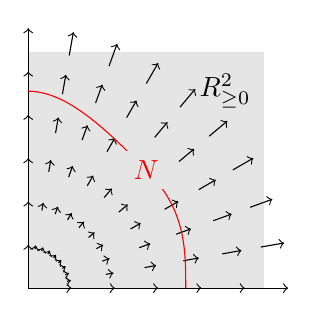
\begin{tikzpicture}
    \fill[gray!20] (0,0)--(3, 0)--(3,3)--(0,3)--cycle;
    \draw (0,0)--(3,0) (0,3)--(0,0);
    \foreach \r in { .5, 1,1.5, 2,2.5, 3} {
        \foreach \t in {0,...,9} {
            \draw[->] ({\r * cos(10*\t)},{ \r * sin(10*\t) })-- ({1.1*\r * cos(10*\t)},{ 1.1*\r * sin(10*\t) });
            }
    }
    
    \draw[red] (0,2.5) .. controls (0.5,2.5) and (1,2) .. (1.5,1.5) node[fill=gray!20] {$N$} .. controls (2,1) and (2,0.5) .. (2,0);
    \node at (2.5, 2.5) {$\mathbb R_{\geq 0}^2$};
    \end{tikzpicture}

%label:"def:reebVectorField"
%author:JeffHicks
%name:"Reeb vector field"
%type:"definition"

 
    Let $(M, \alpha)$ be a contact manifold. The Reeb vector field is the unique vector field $R_\alpha$ characterized by 
    \begin{align*} R_\alpha\in \ker(d\alpha) && \alpha(R_\alpha)=1.\end{align*}
    \label{def:reebVectorField}
 
%label:"exm:reebVectorField"
%author:JeffHicks
%name:"contact hypersurfaces"
%type:"example"
%parent:"exm:contactManifold,exm:reebVectorField"


    We return to \cref{exm:contactManifold} of hypersurfaces in $\RR^{2n}$ given by $M=p^{-1}(N)$. 
    Consider the hypersurface $N$ defined by the equation $p_1+\cdots p_n=1$. Then $M=S^{2n-1}\subset \RR^n$.
    We give $\CC^n$ the polar coordinates $(r_i, \theta_i)$. 

    Let $f=\sum_{i=1}^n |z_i|^2.$ 
    The tangent space to $M$ is the orthogonal complement to $\grad(f).$ Consider the vector field 
    \[V:=\sum_{i=1}^n  x_i \partial_{y_i}- y_i \partial_{x_i}.\]
    First, observe that 
    \[V\cdot \grad(f)=\sum_{i=1}^n( x_i y_i - y_i x_i )= 0 \]
    so $V$ restricts to a vector field on $M$. 
    Let $v=\sum_{i}a_i \partial_{x_i}+b_i\partial_{y_i}$ be any vector in  $TM$. Then the pairing
    \begin{align*}
        \omega(v, V)=&\sum_{i=1}^n a_ix_i+b_iy_i\\
        =&v\cdot \grad(f)=0
    \end{align*}
    From this, we conclude that $V\in \ker(d\alpha)$.
    Finally, we have that $\alpha=\iota_Z\omega$, so 
    \[\omega(Z, V)=\sum_{i=1}^n (x^2+y^2)=1\]
    From which we conclude that $V$ is the Reeb vector field for $(M, \alpha)$.


%define Reeb Orbit
A Reeb orbit is a map $\gamma: \RR/\ell\ZZ\to M$ with $\frac{d}{dt}\gamma = R$. Unlike the setting of Hamiltonian Floer theory, we do not restrict ourselves to time-one orbits. We have a contact-version of the Arnold conjecture.
%tag:000K
%label:"cnj:weinsteinConjecture"
%author:JeffHicks
%name:"Weinstein conjecture"
%type:"conjecture"

 \begin{conjecture}
    Every contact manifold $(M, \alpha)$ has at least one Reeb orbit.
    \label{cnj:weinsteinConjecture}
 \end{conjecture}
Since we do not restrict ourselves to time one-orbits, if there is an orbit, there are an infinite number of orbits (by considering their multiple covers). Even when one considers orbits up to multiplicity, an infinite number of orbits can occur.
%label:"exm:reebOrbits"
%author:JeffHicks
%name:"Reeb orbits on the sphere"
%type:"example"
%parent:"exm:contactManifold,exm:reebVectorField"


    We return to \cref{exm:reebVectorField} of the Reeb vector field on $(S^{n-1},\alpha)$, where $S^{n-1}$ is considered as a hypersurface of $\CC^n$. Recall we have a map $p:S^{2n-1}\to N$, where $N\subset \RR_{\geq 0}^n$ is the simplex defined by $\sum_{i=1}^n p_i^2=1$. The fibers of $p$ are $n$-dimensional tori in $S^{2n-1}$ which are parallel to the Reeb vector field $V_\alpha$. In fact, Reeb vector field $V_\alpha$ acts on the fibers $p^{-1}(p_1, \ldots, p_n)$ by translation in the $(\sqrt p_1, \ldots, \sqrt p_n)$ direction. We therefore identify two types of fibers of $p$:
    \begin{itemize}
        \item If $(\sqrt p_1, \ldots, \sqrt p_n)$ has integral slope (that is, there exists a scalar $r$ so that $r\cdot(\sqrt p_1, \ldots, \sqrt p_n) \in \ZZ^n$) then every point on the fiber belongs to a closed orbit.
        \item Otherwise, no point on the fiber belongs to a closed orbit. 
    \end{itemize}
    The Reeb orbits of $(S^{n-1}, \alpha)$ are in bijection with $\bigoplus_{\vec v\in \NN^n\setminus \{0\}} T^n/\vec v$.



In \cref{exm:reebOrbits} we have an uncountable number of orbits, but the set of periods of these orbits is only countable.  Given a Reeb orbit $\gamma$, let $\ell(\gamma)$ denote its period.
%label:"prp:countableNumberOfReebPeriods"
%author:JeffHicks
%name:"periods of Reeb orbits"
%type:"proposition"

 
    Let $M$ be a contact manifold. Let 
    \[\Gamma:=\{\gamma: \RR/\ell\RR\to M \st\gamma'=R\}\]
    denote the set of Reeb orbits. The image of $\ell(\Gamma)\subset \RR_{\geq 0}$ is countable and closed.
    \label{prp:countableNumberOfReebPeriods}
 
%tag:000T
%parent:prp:countableNumberOfReebPeriods
%label:"prf:countableNumberOfReebPeriods"
%author:JeffHicks
%name:"periods of Reeb orbits"
%type:"proof"

    Give a Reeb orbit, the reparameterization of the orbit satisfying $\dot \gamma = \ell V_\alpha$ is a critical point of the action 
    \begin{align*}
        A:W^{1,2}(S^1, M)\to& \RR\\
        \gamma\mapsto& \int_{\gamma}\alpha
    \end{align*}
    where $W^{1,2}(S^1, M)$ is the space of maps of Sobelov class $1,2$.
    On a Reeb orbit, observe that 
    \[\int_{\gamma}\alpha= \int_{S^1} \alpha(\cdot \gamma) = \ell\]
    the action computes the period of $\gamma$. Therefore the set of periods is a subset of the critical values of $A$. By applying the Sard-Smale theorem, the critical values of a functional are countable and closed in $\RR$.

While the Weinstein conjecture is stated in terms of contact geometry, there is a standard method to translate questions in contact geometry to questions in symplectic geometry.
%label:"def:symplectization"
%author:JeffHicks
%name:"symplectization of a contact manifold"
%type:"definition"

 
    \label{def:symplectization}
    Let $(M, \alpha)$ be a contact manifold. The symplectization of $(M, \alpha)$ is the symplectic manifold
    \[(\RR\times M, d(\exp(r)\cdot \alpha)).\]
 
%label:"rem:symplectization"
%author:JeffHicks
%name:"symplectization of a contact manifold"
%type:"remark"
%parent:def:symplectization

 
    To see that this is a symplectic manifold, observe that 
    \begin{align*}
        (d(\exp(r)\cdot \alpha)^n=( \exp(r) (dr\wedge\alpha + d\alpha))^n = \exp(nr) ( dr\wedge \alpha\wedge d\alpha^{n-1})
    \end{align*}
    which is non-vanishing everywhere as $\alpha$ is a contact form.
 
%label:"def:linearHamiltonian"
%author:JeffHicks
%name:"linear Hamiltonian"
%type:"definition"

 
 Let  $M$ be a contact manifold, and let $\RR\times M$ be its symplectization. A \emph{linear Hamiltonian} of slope $m$ is the Hamiltonian $H^m(r, x)= m\cdot \exp(r)$.
 \label{def:linearHamiltonian}
 
%tag:000K
%label:rem:linearHamiltonian
%author:JeffHicks
%name:"linear Hamiltonian"
%type:remark
%parent:def:linearHamiltonian

 

Observe that the level sets of a linear Hamiltonian are  $\{r\}\times M$. The Hamiltonian vector field therefore can be restricted to a vector field on the contact manifold $M$. It is not a surprise that the $m V_\alpha$ and Hamiltonian vector field $H_V$ agree:
\begin{align*}
    \iota_{i_* m V_\alpha}\omega=& d(\exp(r) \alpha )(m V_\alpha)\\
     =&(\exp(r) dr \wedge d\alpha - \exp(r) d\alpha) (m V_\alpha)\\
    =&- m \cdot \exp(r)dr = dH^m
\end{align*}
Therefore, the time one Hamiltonian orbits of $H$ correspond to the time $m$ Reeb orbits of $V_\alpha$; by studying Hamiltonian Floer theory on the symplectization $\RR\times M$ we obtain some understanding of the Reeb dynamics of $(M, \alpha)$.

Alternatively, if $m$ is not a period of some Reeb orbit, Then $\RR\times M$ has no time one orbits for the linear Hamiltonian of slope $m$. 
 
%tag:000K
%label:rem:increasingHamiltonian
%author:JeffHicks
%name:"orbits of an increasing Hamiltonian"
%type:remark

 
   \label{rem:increasingHamiltonian}
    If we take $h: \RR_{\geq 0}\to \RR$ a function with slope increasing to infinity the Hamiltonian $H:=h(\exp(r)): X\times \RR\to \RR$ our Hamiltonian vector field is related to the linear Hamiltonian vector fields by  
    \[V_H = h'(\exp(r)) V_{H^1}\]
    Therefore, the time-one Hamiltonian orbits contained in the level set $\exp(r)\times M$ will compute the $h'(\exp(r))$-period Reeb orbits of $V_\alpha$.
 